
\chapter[Metodologia]{Metodologia}
  Esse capítulo irá apresentar quais métodos serão utilizados para que o trabalho
atinja os objetivos finais.
%%%%%%%\section{Resumo do Capítulo}

\section{Metodologia de Condução do Trabalho de Conclusão de Curso}
\label{Sec:MetCondTCC}
%Revisão bibliografica (contexto biomedica)
%Trabalho do Roberto - compreender o que foi feito e como foi feito (levantar os componentes funcionais do sistema)
%Tecnologia - aprender (unity + python + matlab)
%prototipos conceitos -- python (arquivos + dados) + unity
%levantamento de requisitos  (historias de usuario)
%escrita TCC1
%implementação das historias
%testes
%integração
%build
%escrita tcc2
  Neste capítulo será apresentada a metodologia inicial que deverá ser adotada
para o desenvolvimento deste trabalho, podendo ser ratificado após a escrita do
trabalho de conclusão de curso 2.

  Este trabalho foi baseado no exame de qualificação do Roberto \cite{roberto}.
e podemos afirmar que ele pertence a área da engenharia biomédica. "Classicamente, 
a Engenharia Biomédica é vista como a aplicação dos métodos de distintas áreas 
das Ciências Exatas e de Engenharia no campo das Ciências Médicas e 
Biológicas."\cite{engenhariaBiomedica}. Pois ele desenvolve uma abordagem 
inovadora aplicado a terapia de  doenças/acidentes motores, ou seja, aplicado a
 fiosioterapia. Onde desenvolve uma nova abordagem para análise de movimentos.

  Para o desenvolvimento deste trabalho, serão necessárias conversas com 
o autor para esclarecimento do escopo, da aplicação do trabalho e para a compreensão
do protótipo e seu código fonte, desenvolvido por ele no matlab junto ao exame. 
Além disso, faz se necessário o uso da engenharia reversa para identificar os 
principais módulos funcionais do protótipo e com isso levantar os requisitos, 
que será por meio de histórias de usuário, então assim desenvolvendo e 
implementando as funcionalidades para a familiarização com a tecnologia e o 
desenvolvimento do trabalho de conclusão de curso.
  
  %Carla: deixar claro a metodologia do TCC: Conversas com o autor para esclarecer o escopo e a aplicação do trabalho. Compreensão do código fonte do protótipo desensvolvido pelo autor no matlab
  % Engenharia reversa para identificar os principais módulos funcionais do protótipo, levantamento dos requisitos por meio de histórias de usuário, implementação de funcionalidades para 
  %familiarização com a tecnologia, escrita do tcc
  
   Este trabalho está propondo transformar o exame de qualificação \cite{roberto}
em produto, para isto é essencial usar uma linguagem mais difundida e com mais 
suporte para processamento de sinais, para esta função foi escolhido a
linguagem python, e para a interface humano computador o Unity 3D\cite{unity3d}. 
Para o devido desenvolvimento, necessitará de uma fase de aprendizado de ambas 
as tecnologias, além do aprendizado do uso do software matlab, para o correto
entendimento do protótipo desenvolvido no exame de qualificação. Os recuros 
usados serão o manual do Unity 3D \cite{unity3dManual}, a documentação do 
Python 3 \cite{pythondoc} e a documentação do Matlab \cite{matlabdoc}, além de 
fóruns online.

\section{Protótipo}
\label{Sec:protótipo}
  Junto com o exame de qualificação citado anteriormente \cite{roberto}, foi 
desenvolvido um protótipo no software matlab \cite{matlab}. Esse sistema inicial
implementou algumas das teorias do exame. Ele possui três etapas: rotular os dados,
parametrização e utilizar para segmentação automática.
\begin{itemize}

\begin{sloppypar}

\item \textbf{Rotulação}: Na etapa de rotular os dados,começando pelo arquivo
' SCRIPT\_labelAndIndexMultivariateFile\_WBM21.m '. Neste script estão duas funções, 
\textit{labelAndIndexUnivariateFile} que por sua vez chama a função 
\textit{labelAndIndexUnivariateStructDataset} que chama a função \textit{labelAndIndexUnivariateDataset}
e \textit{transitionIndexMultivariateFile}.Os dados de entrada são puxados dos arquivos da pasta 
'PreProcessedData','/',DecRateN\_Filter,'/',Movement,'/',Subject,'/',Trial,'.mat'.
Esses dados foram coletados previamente por sensores. Os dados são uma struct .mat
com  os ângulos de algumas articulações e o tempo. Esses ângulos são dados em radianos
 e são divididos em articulações e em uma única coluna como podemos observar em \ref{structMatlab}.

\begin{figure}[!h]                                                               
\centering                                                                         
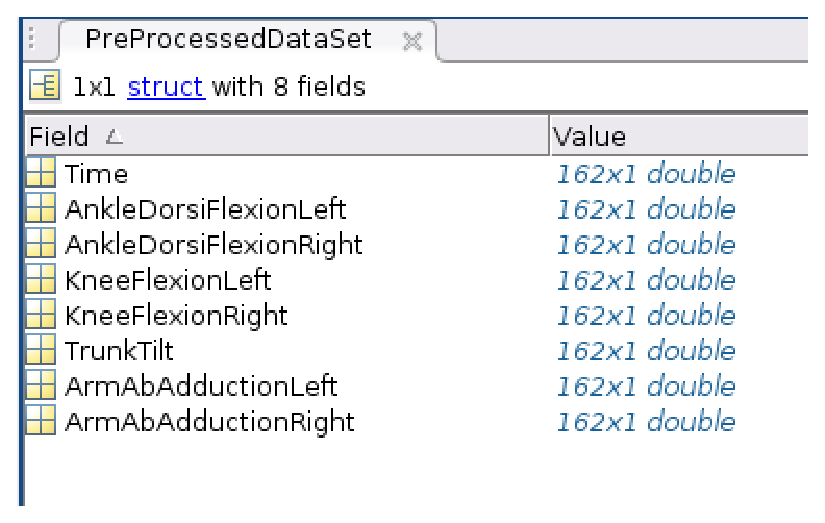
\includegraphics [keepaspectratio=true,scale=0.60]{figuras/structMatlab.eps}                                
\caption{Dados das articulações}                                        
\label{structMatlab}                                                        
\end{figure} 

  Quando o script é executado  primeiro um gráfico é traçado com várias curvas 
 para selecionar o início e fim de cada conjunto de dados,
depois cada curva é apresentada separadamente. Essa é a etapa para rotular os 
dados de cada curva. No prompt ele pergunta qual o “\textit{Switch Variable}”, em seguida
 ele pede para marcar  o início e o fim do intervalo com esse rótulo. A seguir 
pergunta se é o fim do  conjunto de dados. Caso não seja o fim ele volta a
 perguntar qual a “Switch Variable”. Esse procedimento se repete para todas as curvas.
Logo após, vem a parte que rotula os dados multivariáveis dependendo do conjunto 
de rótulos de cada variável separada. O resultado é a struct “thisLabeledIndexStructDataSet” salvo na pasta 
LabeledDataMultivariate’/‘,DecRateN\_Filter,'/',Movement,'/',Subject,'/',Trial,'.mat'.

\item \textbf{Parametrização}: Na etapa de parametrização do modelo a função:
 \"SLDS\_Univariate\_ParameterDataSetBuilder2.m\" pega os dados rotulados da etapa 
anterior, ou seja os dados segmentados automaticamente e com as funções 
“parametersCteVelSpaceStateModel2” e “hmmTransitionMatrix2” calcula os parâmetros 
do Modelo Oculto de Markov. Esta função é a base para o script 
"SLDS\_Univariate\_IntraSubject\_ParameterDataset\_Script.m”  que pega diversos
 conjuntos de dados rotulados, de diferentes sujeitos ou diferentes execuções 
do mesmo sujeito e chama a função “SLDS\_Univariate\_ParameterDataSetBuilder2.m”
 para cada um deles e no fim temos os parâmetros do modelo oculto de Markov ajustado
 para vários conjuntos de treinamento.  

\end{sloppypar}
\item \textbf{Segmentação}: Esse é o programa que faz a estimação dos rótulos associado com cada medida. 
A principal função é a “SLDS\_Filter\_Univariate” ela recebe as structs 
ValidationTrialThisVariable e FittedModelThisVariable e a variável 
InitialSwitchVariableState. A ValidationTrialThisVariable contém os dados a serem
 classificados e pode conter também os rótulos. São as medidas do movimento, os 
mesmos dados usados na parte de rotulação. O FittedModelThisVariable são todos 
os parâmetros do modelo (análogo aos parâmetros do ModeloOculto de Markov). 
A variável InitialSwitchVariableState indica o símbolo da primeira medida.

Na imagem \ref{diagramProt} podemos ver todo o fluxo de dados do protótipo.
\end{itemize}

\begin{figure}[!h]                                                           
\centering                                                                   
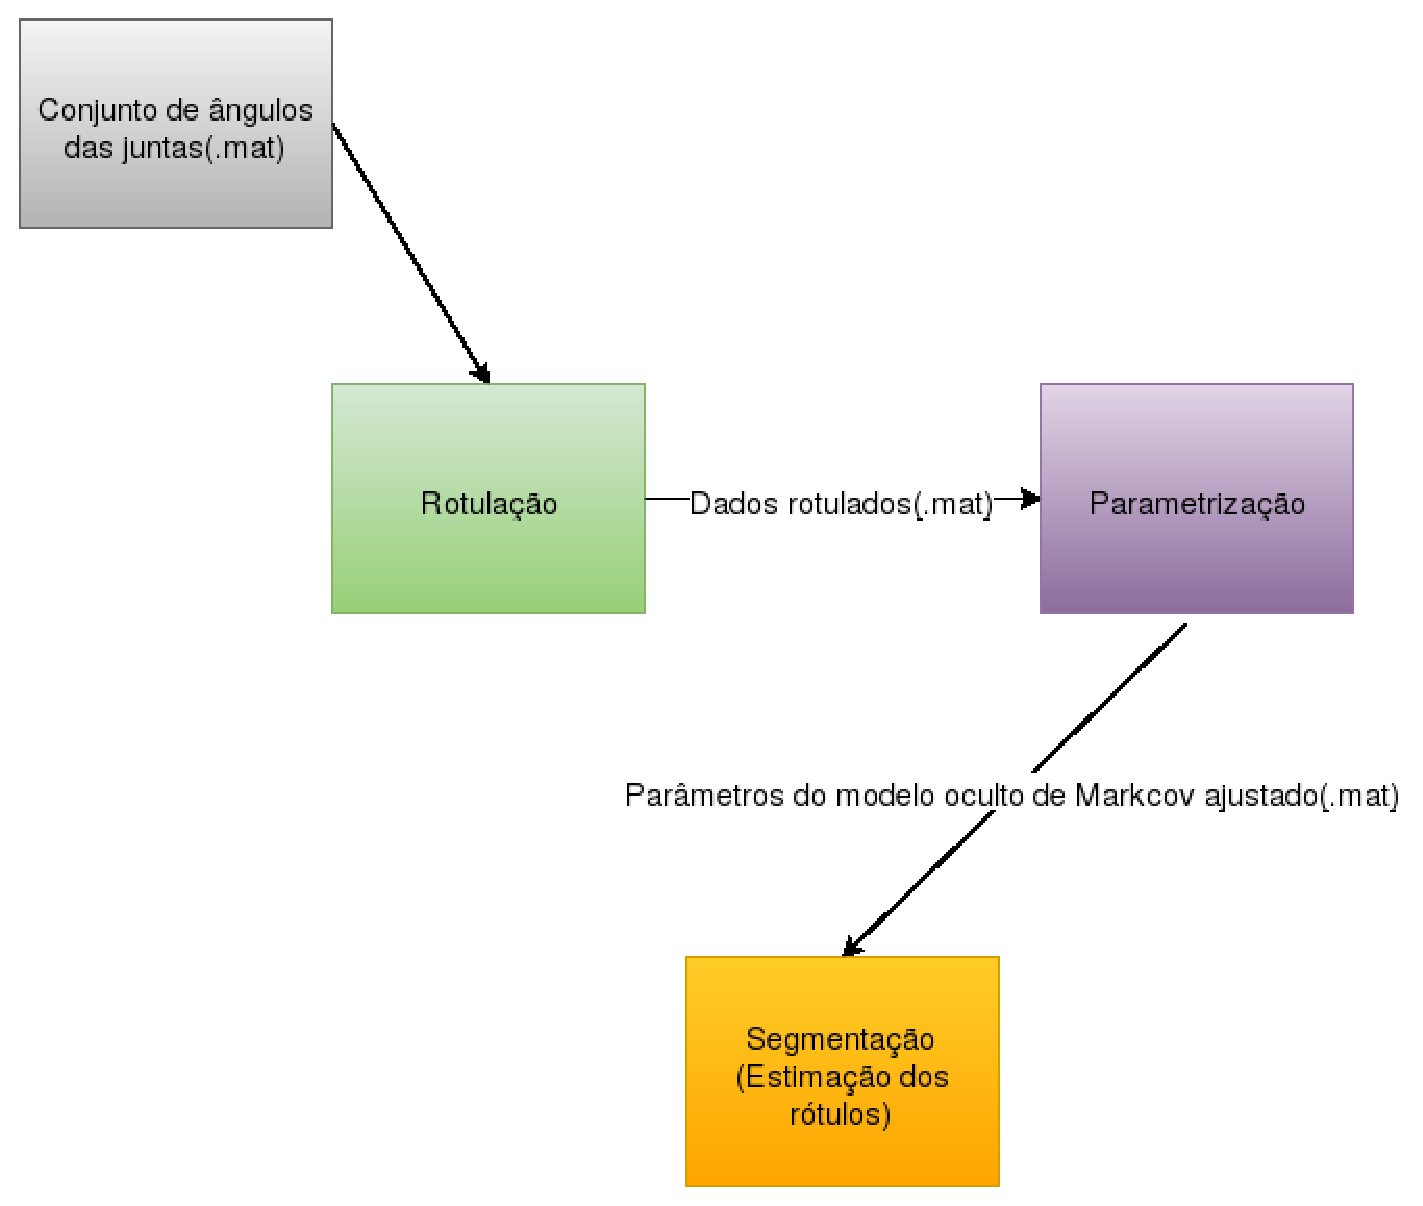
\includegraphics [keepaspectratio=true,scale=0.60]{figuras/diagramProt.eps} 
\caption{Fluxo de Dados}                                   
\label{diagramProt}                                     
                                                                             
\end{figure}                                                                 
 

\section {Requisitos}
\label{Sec:Requisitos}
  Um requisito é definido como "uma condição ou uma capacidade com a qual o 
sistema deve estar de acordo"\cite{requisitos}. Existem vários tipos de 
requisitos. Um modo de categorizá-los é descrito como o modelo 
FURPS+\cite{robertGrady} , seguindo esse modelo, elicitamos os requisitos 
iniciais do sistema: 
  \begin{itemize}
  \item \textbf{Funcionalidade}(Functionality):
    \begin{itemize}
    \item Software para auxilar o acompanhamento de pacientes em reabilitação 
    motora de movimentos específicos.
    \item É realizado por meio de comparação do movimento preciso das articulações do
     corpo humano em tempo real, com uma base de articulações com os movimentos 
    previamente estabelicidos.
    \item Apresenta um conjunto de movimentos gravados para seleção e execução.
    \end{itemize}
  \item \textbf{Usabilidade}(Usability)
    \begin{itemize}
    \item O usuário do sistema será capaz de visualizar todo tipo de informação
     textual, imagem ou modelo 3d na aplicação , com clareza, em qualquer 
    monitor independente de resolução.
    \item Documentação ampla e de fácil compreensão, abordando todas as 
    funcionalidades disponível na aplicação.
    \end{itemize}
\item \textbf{Confiabilidade}(Reability)
    \begin{itemize}
    \item O sistema será capaz de verificar algum erro ou inconstância entre os
     dados recebidos dos sensores, podendo assim se recuperar ou informar 
    alguma falha na comunicação com os mesmos.
    \end{itemize}
\item \textbf{Desempenho}(Performance)
    \begin{itemize}
    \item O sistema analisará o movimento exato feito pelo usuário em tempo real.
    \end{itemize}
\item \textbf{Suportabilidade}(Supportability)
    \begin{itemize}
    \item Para que alcance um maior número de usuários e para que não seja exclusivo de um sistema operacional,
 inicialmente é desejável que seja suportável em qualquer computador pessoal, que tenha como sistema
     operacional alguma distribuição linux ou windows.
    \item Possuir uma suíte de testes sendo eles de aceitação e unitário.
    \end{itemize}
  \end{itemize}

\subsection{Histórias de usuário}
\label{Sec:Histórias de usuário}
  Como prática ágil as \textit{User stories}(Histórias de usuário), são artefatos
de desenvolvimento, utilizadas para organizar requisitos. Tem-se foco nos objetivos
do usuário e como o sistema alcança esses objetivos.
  
  Para melhor organizar e fracionar os requisitos deste trabalho, foi adotado 
essa prática ágil, podemos ver um levantamento inicial do \textit{product backlog} \ref{historias}
%Carla: cadê as histórias de usuários?
\begin{table}[]
\centering
\caption{Histórias}
\label{historias}
\begin{tabular}{|l|l|}
\hline
\textbf{História} & 1                                                        \\ \hline
\textbf{Eu como}  & Usuário administrador(fisioterapeuta)                    \\ \hline
\textbf{Desejo}   & Visualizar os dados obtidos das articulações                   \\ \hline
\textbf{Para}     & poder identificar movimentos desejados e assim rotulá-lo \\ \hline
 \multicolumn{2}{|l|}{}                                                       \\ \hline
\textbf{História} & 2                                                        \\ \hline
\textbf{Eu como}  & Usuário administrador                                    \\ \hline
\textbf{Desejo}   & Visualizar a movimentação em um avatar 3D                \\ \hline
\textbf{Para}     & Poder certificar a rotulação de dados da movimentação da articulações\\ \hline
\multicolumn{2}{|l|}{}                                                       \\ \hline
\textbf{História} & 3                                                        \\ \hline
\textbf{Eu como}  & Usuário administrador                                    \\ \hline
\textbf{Desejo}   & Que o sistema corrija minha movimentação em tempo real   \\ \hline
\textbf{Para}     & Poder melhor executar os movimentos das articulações           \\ \hline
\multicolumn{2}{|l|}{}                                                       \\ \hline
\textbf{História} & 4                                                        \\ \hline
\textbf{Eu como}  & Usuário administrador(fisioterapeuta)                    \\ \hline
\textbf{Desejo}   & Que o sistema salve um novo movimento                    \\ \hline
\textbf{Para}     & Poder constar no catálogo do sistema e poder ser executado \\ \hline
\multicolumn{2}{|l|}{}                                                       \\ \hline
\textbf{História} & 5                                                        \\ \hline
\textbf{Eu como}  & Usuário                                                  \\ \hline
\textbf{Desejo}   & Visualizar o movimento a partir de um catálogo           \\ \hline
\textbf{Para}     & Poder escolher o movimento correto                       \\ \hline
\multicolumn{2}{|l|}{}                                                       \\ \hline

\textbf{História} & 6                                                        \\ \hline
\textbf{Eu como}  & Usuário                                                  \\ \hline
\textbf{Desejo}   & Desejo escolher movimento de referência                  \\ \hline
\textbf{Para}     & Melhor seguir receita médica                             \\ \hline
\multicolumn{2}{|l|}{}                                                       \\ \hline

\textbf{História} & 7                                                        \\ \hline
\textbf{Eu como}  & Usuário                                                  \\ \hline
\textbf{Desejo}   & Feedback do movimento sendo executado                    \\ \hline
\textbf{Para}     & Poder melhor executar os movimentos das articulações           \\ \hline
\multicolumn{2}{|l|}{}                                                       \\ \hline

\textbf{História} & 8                                                        \\ \hline
\textbf{Eu como}  & Usuário                                                  \\ \hline
\textbf{Desejo}   & Salvar meu movimento real                                \\ \hline
\textbf{Para}     & Poder ver meu progresso                                  \\ \hline
\multicolumn{2}{|l|}{}                                                       \\ \hline
\end{tabular}
\end{table}


%% Carla: SalvaR Movimento ou catalogar um novo movimento - administrador -- Visualizar movimento a partir de um catalogo -- escolher movimento de referencia ativo (para ser executado) --
%% comparar o movimento ativo com o movimento real -- dar feedback do movimento -- salvar movimento real. Processamento sinal roberto

  Como já citado anteriormente, tais histórias serão implementadas com as tecnologias
python para processamento de sinais e Unity 3D para visualização, onde será 
estudado a melhor forma para integração de ambas as tecnologias. Cada história
se dará por completa quando devidamente implementada e possuindo sua suíte de testes
unitários e de aceitação.

\section{Metodologia Adotada no Desenvolvimento da Ferramenta}
%scrum adaptado - práticas 
%testes aceitação
%arquitetura do sistema

%Carla: deixa explicito como será feito os artefatos. Ex: backlog vai ficar no zenhub/trello? como pode ser feito o acompanhamento do trabalho?
%sprints: duas semanas. Tempo necessário para cada um dos rituais (sprint planning etc). Definição de pronto: quando uma feature está pronta? quando 
% tiver X cobertura (integração contínua??) e funcionalidade aprovada pelo PO. Condições para entrega
  Iremos adotar algumas práticas e artefatos da  metodologia 
scrum (\ref{Sec:Scrum}) para gerenciamento, e do extreme programming - XP (\ref{Sec:xp}
para desenvolvimento), nesta seção iremos descrever tais artefatos e práticas, 
além dos papéis envolvidos.

  Para o \textit{Product Backlog}  usaremos a ferramenta trello. Trello é uma ferramenta
de gerenciamento de projetos que pode ser ajustada de acordo com as necessidades
do usuário. O \textit{Product Backlog} estará disponível inicialmente somente para
os envolvidos neste trabalho.

  As \textit{Sprints} terão duração de duas semanas. Já as \textit{Sprints Plannings}
e as \textit{Sprints reviews}, terão durações de no máximo uma hora e serão 
discutidas com os responsáveis por desempenhar os papéis de \textit{Product Owner}.

  Para \textit{Definition of Done}, uma feature só será considerada pronta quando
devidamente testada e também após ser aprovada pelos \textit{Product Owners}, que 
será desempenhado pelos orientadores deste trabalho.
  
  Para versionamento do código, será utilizado o bitbucket, que se trata de um
repositório de projetos baseado no sistema Git de controle de versão.

\subsection{Arquitetura do sistema}
\label{Sec:arquitetura}
%Colocar aqui os principais módulos funcionais do sistema. A arquitetura proposta (com os modulos) e como será feita a comunicação entre os módulos
  De acordo com a ISO/IEEE 1471-2000 - Arquitetura é a organização fundamental 
de um sistema incorporada em seus componentes, seus relacionamentos com o 
ambiente, e os princípios que conduzem seu design e evolução.Para este sistema 
foi definido a arquitetura conhecida como arquitetura por componentes.
  
  De acordo com Brown e Wallnau \cite{brownWall}, um componente é 
"uma não-trivial, quase independente, e substituível parte de um sistema que 
cumpre uma função clara no contexto de uma arquitetura bem definida".

  O sistema proposto por esse trabalho, inicialmente terá quatro grandes módulos,
 sendo eles:

  \begin{itemize}
  \item Módulo do sensor: Responsável pela aquisição de dados do movimento do 
  usuário;
  \item Módulo do processamento de sinal: Responsável pelo processamento dos dados
  adquiridos pelo módulo anterior;
  \item Módulo de visualização: Responsável pela interface com o usuário;
  \item Módulo do banco de dados: Responsável por guardar as informações das articulações.
  \end{itemize} 

  A comunicação entre o módulo sensor e o módulo processamento, será por meio 
das informações das articulações colhidas pelos sensores e enviadas para o processamento.
O módulo do processamento se comunicará, além do módulo do sensor, com os demais
módulos, a troca com o módulo de visualização será de  informações sobre as articulações,
e o estado da movimentação, podendo estar de acordo com a base de dados ou não e 
dizendo onde se encontra os erros de execução. Já a comunicação com o módulo do
banco de dados será por meio de informações de articulações, podendeo ser já catalogadas
 ou o cadastro de novos movimentos. Podemos melhor enxergar essa comunicação na 
figura \ref{diagrama}

\begin{figure}[!h]                                                           
\centering                                                                   
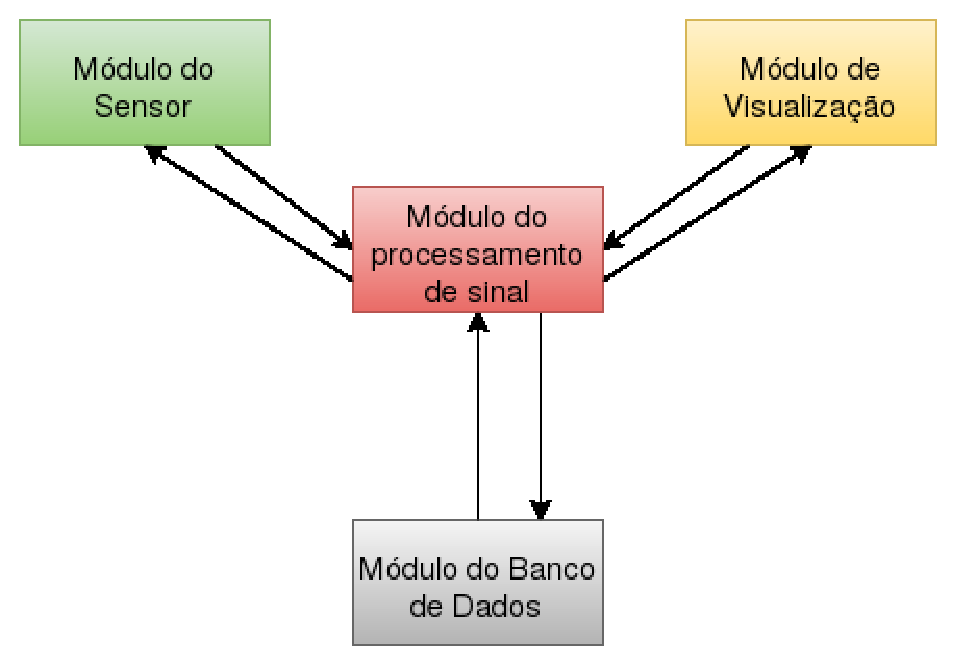
\includegraphics [keepaspectratio=true,scale=0.60]{figuras/diagrama.eps} 
\caption{Diagrama de Arquitetura}                                   
\label{diagrama}                                     
                                                                             
\end{figure}                                                                 
  
\subsection{Planejamento das atividades}
\label{Sec:Planejamento}
  Para esta seção, iremos apresentar um cronograma inicial para as atividades
até a conclusão deste trabalho. Cronograma  é uma representação de um plano de 
execução das atividades do trabalho, incluindo durações, dependências, e outras 
informações de planejamento.

\begin{figure}[!h]                                                           
\centering                                                                   
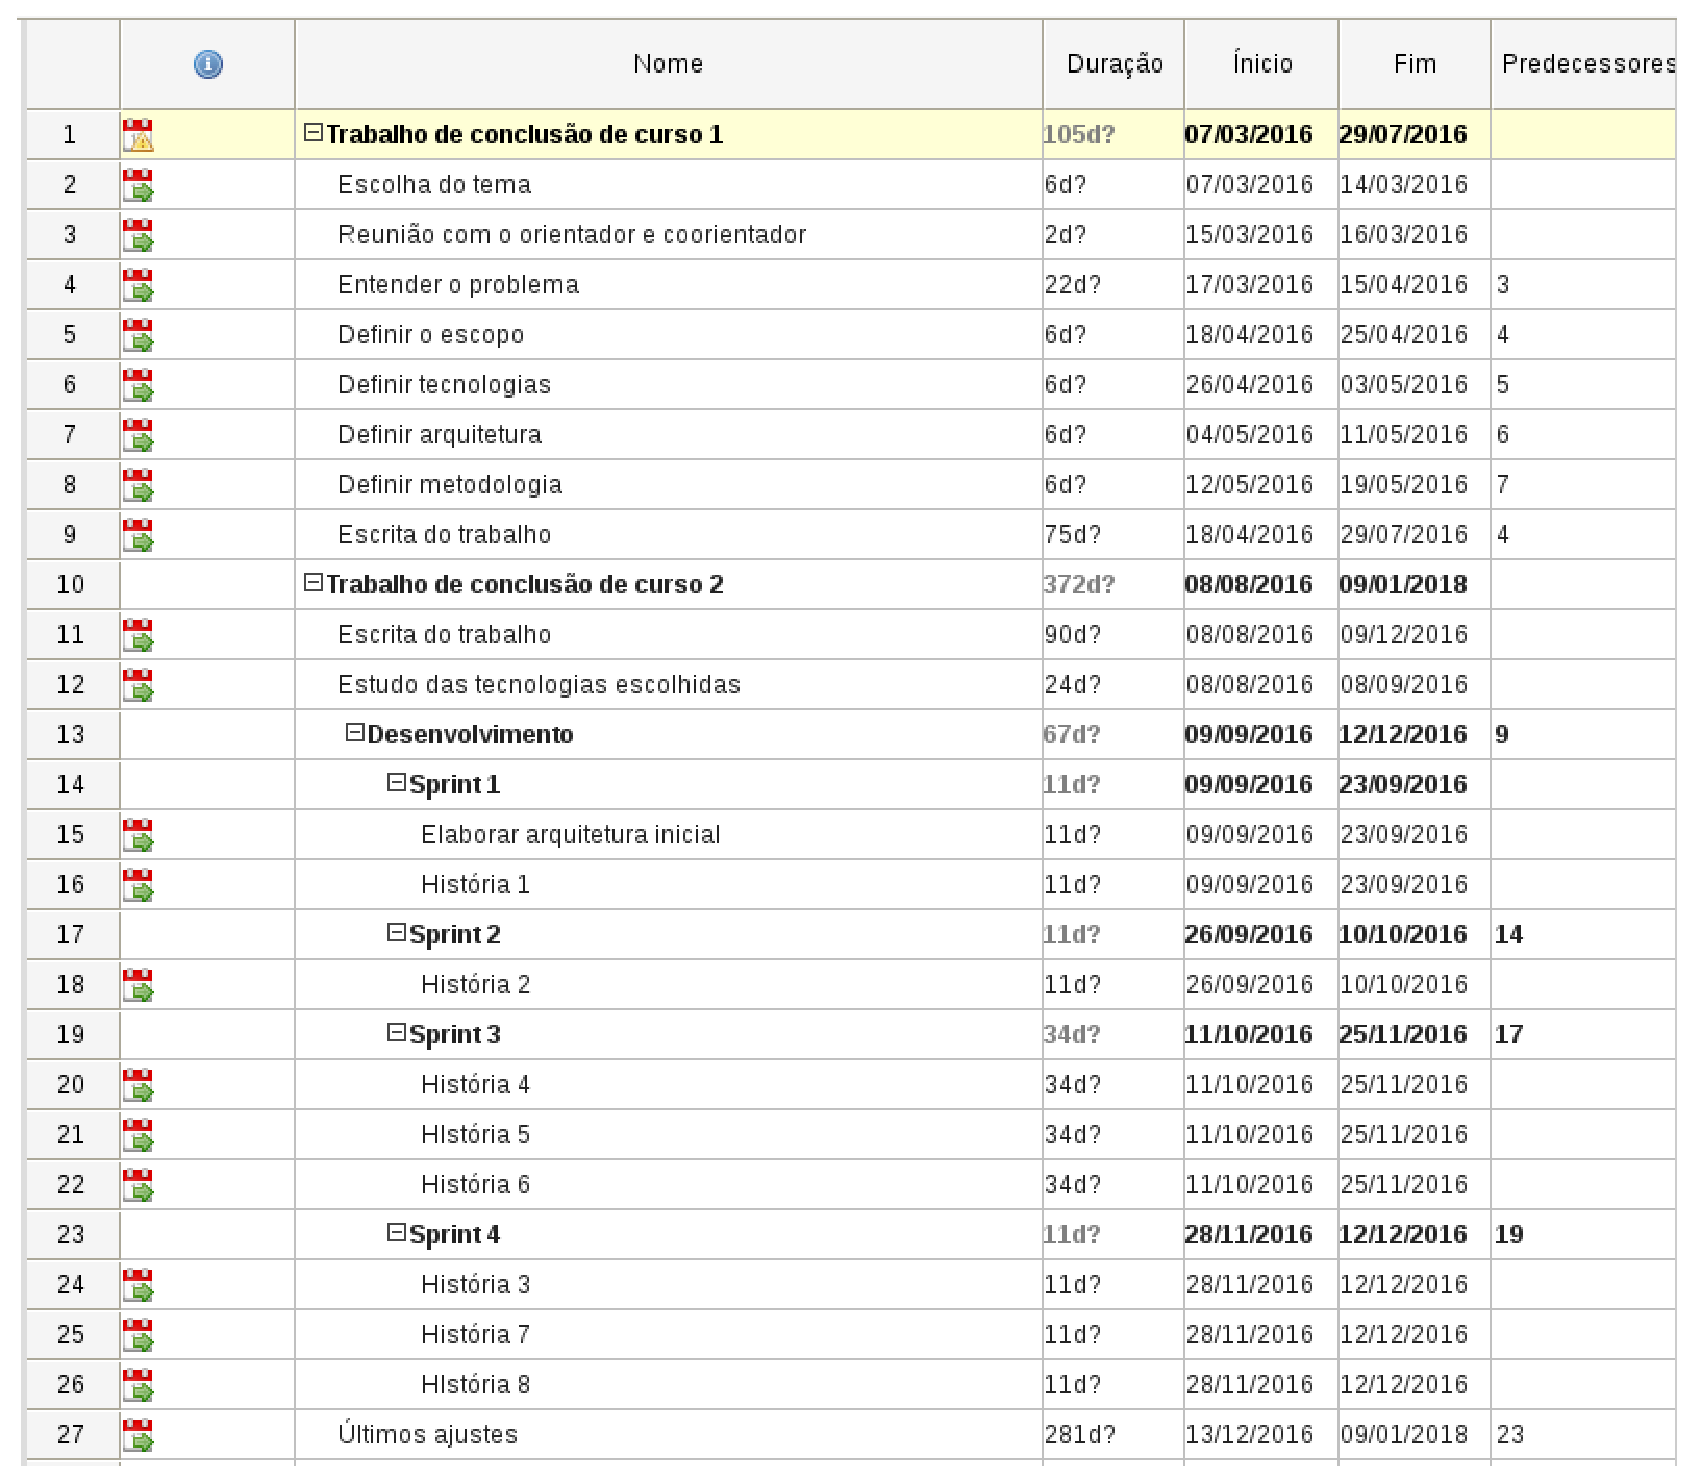
\includegraphics [keepaspectratio=true,scale=0.5]{figuras/diagramaGantt3.eps} 
\caption{Resumo do planejamento das atividades}                                   
\label{resumoDoPlanejamento}                                                                                                                  
\end{figure}                                                                 



\begin{landscape}

\begin{figure}[!h]                                                           
\centering                                                                   
\includegraphics [keepaspectratio=true,scale=0.5]{figuras/diagramaGantt1.eps} 
\caption{Diagrama de Gantt 1}                               
\label{diagramaGantt1}                                                                                                           
\end{figure}                                                                 

\end{landscape}


\begin{landscape}

\begin{figure}[!h]                                                           
\centering                                                                   
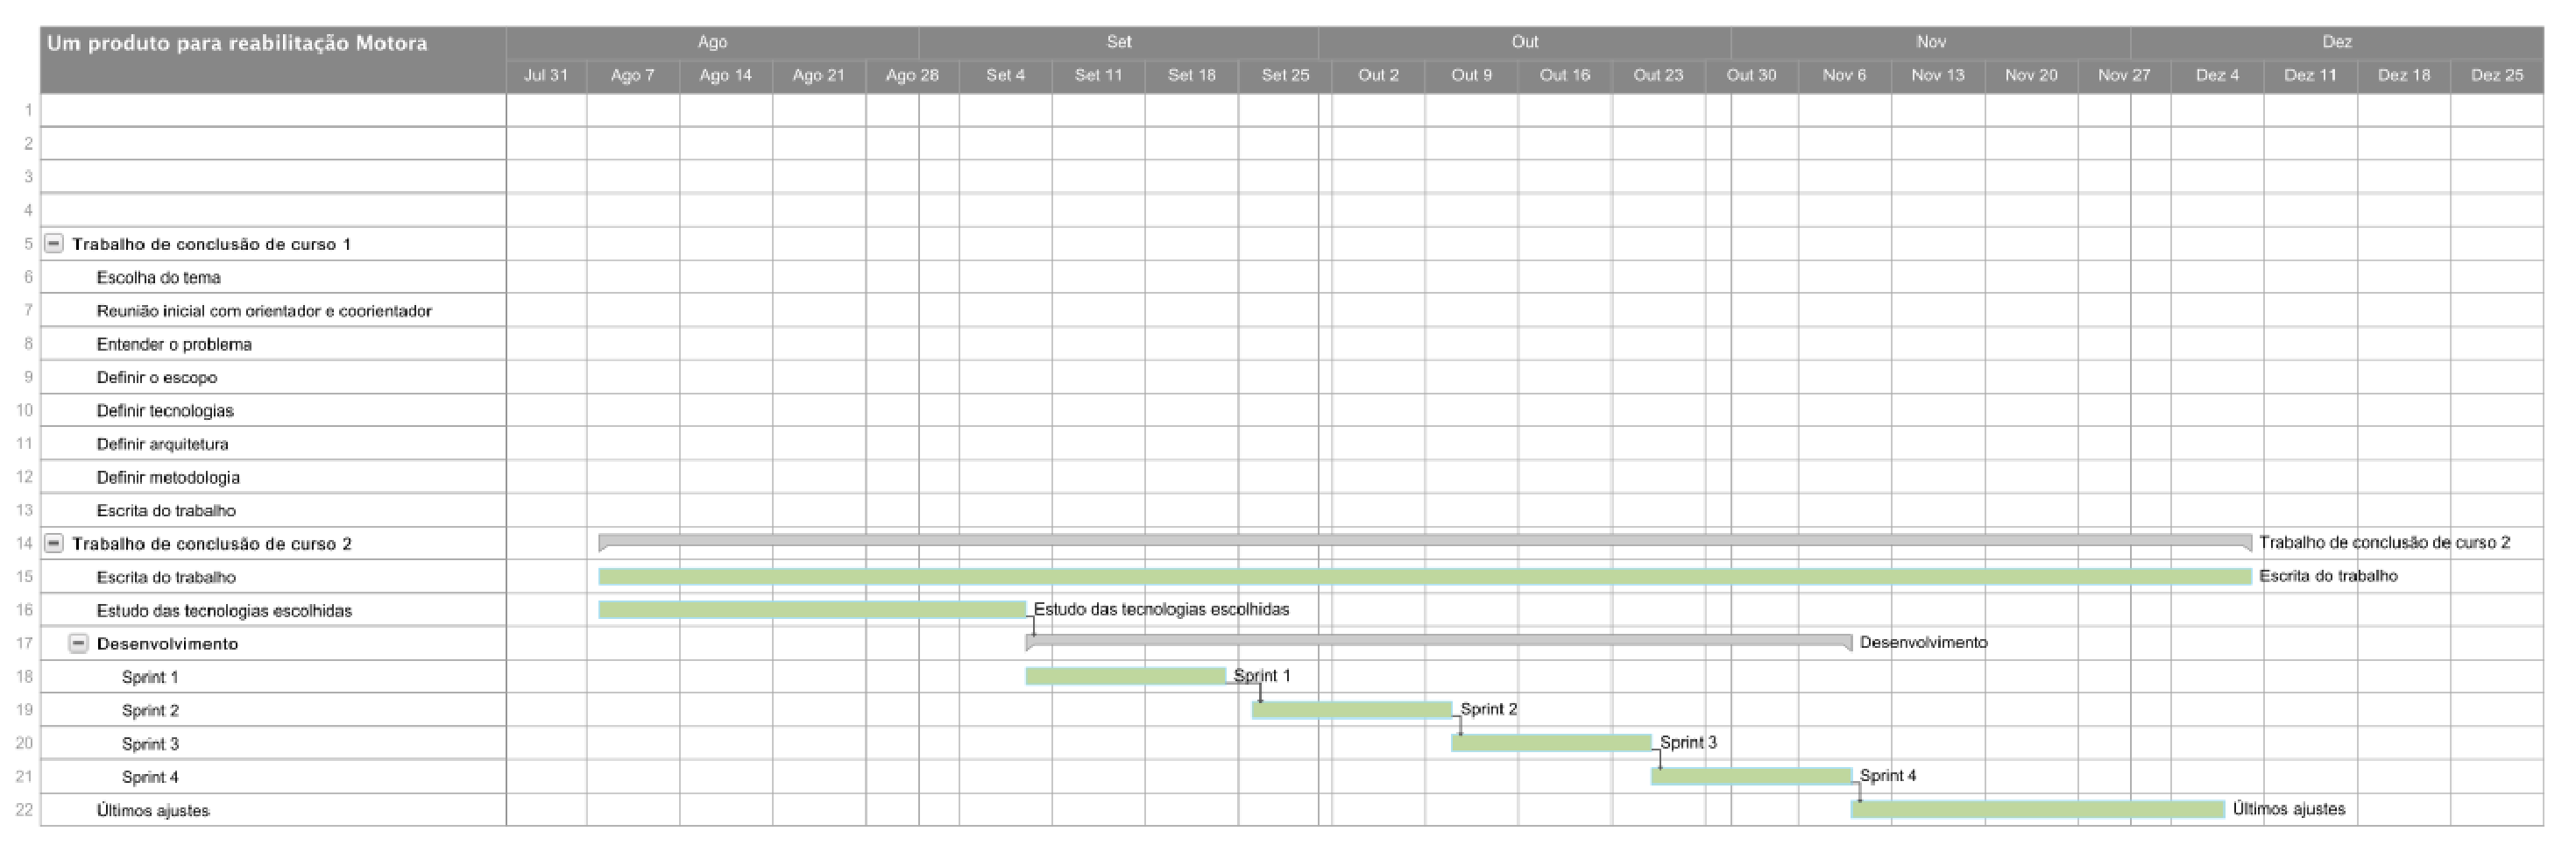
\includegraphics [keepaspectratio=true,scale=0.5]{figuras/diagramaGantt2.eps} 
\caption{Diagrama de Gantt 2}                                   
\label{diagramaGantt2}                                                                                                                  
\end{figure}                                                                 

\end{landscape}


